%-----------------------------------------------------------------------
%
%   UFRJ  - Universidade Federal do Rio de Janeiro
%   COPPE - Coordena��o dos Programas de P�s-gradua��o em Engenharia
%   PEE   - Programa de Engenharia El�trica
%
%   COE-835  Controle adaptativo
%
%   Relat�rio da simula��o
%                                                         Ramon R. Costa
%                                                         05/out/09, Rio
%-----------------------------------------------------------------------
\documentclass[11pt,a4paper]{article}
\usepackage[latin1]{inputenc} %pacote para utilizar palavras acentuadas
\usepackage{amsmath,amssymb}  %pacotes do AMS
\usepackage{latexsym}         %pacote para incluir s�mbolos (ex.\Box)
\usepackage{fancybox,fancyhdr}%pacote com frescuras
\usepackage{graphicx}         %pacote para incluir figuras tipo eps
\usepackage[portuguese]{babel}
\usepackage{xcolor}
\usepackage{float} 
\usepackage{epstopdf}
\usepackage[inline]{enumitem}
\usepackage[a4paper]{hyperref}% Make sure it comes last of your loaded packages
\hypersetup{
  verbose,
  plainpages=false,
  bookmarks=true,
  colorlinks=true,
  linkcolor=blue
}
   
%----------------------------------------------------------------------
%
%   Macros utilizados no LATEX
%                                                       Ramon R. Costa
%                                                       13/out/17, Rio
%----------------------------------------------------------------------
\newcount\m
\newcount\n

\def\twodigits#1{\ifnum #1<10 0\fi \number#1}

\def\hours{\n=\time \divide\n 60
    \m=-\n \multiply\m 60 \advance\m \time
    \twodigits\n:\twodigits\m}

\def\hora{\hours}

\def\fim{
  \medskip
  \begin{center}
    \rule[1mm]{30mm}{0.14mm}$\diamond$\rule[1mm]{30mm}{0.14mm}
  \end{center}
}

%----------------------------------------------------------------------
% A4 paper size & margins
\setlength {\textheight}    {25cm}%
\setlength {\textwidth}     {17.5cm}%
\setlength {\parindent}     {0mm}%
\setlength {\parskip}       {1mm}%
\setlength {\topmargin}     {-14mm}%
\setlength {\oddsidemargin} {-6mm}%
\setlength {\evensidemargin}{-6mm}%
\setlength {\columnsep}     {6mm}%

%----------------------------------------------------------------------
\def\codigo{COE-835}
\def\disciplina{Controle adaptativo}
\def\periodo{3o. período/2017}
\def\professor{Ramon}

\newcommand{\BOX}[1]{
  \framebox{{\color{magenta}\rule[-3mm]{1mm}{9mm}} ~~$\displaystyle
  \begin{aligned} #1 \end{aligned}$~~}\pagestyle{plain}
}

\newcommand{\RED}[1]{\colorbox{white}{\textcolor{red}{#1}}}
%\newcommand{\WoR}[1]{\colorbox{red}{\textcolor{white}{#1}}}
\newcommand{\BLU}[1]{\colorbox{white}{\textcolor{blue}{#1}}}
\newcommand{\GRE}[1]{\colorbox{green}{\textcolor{black}{#1}}}
\newcommand{\HI}[1]{\colorbox{yellow}{\textcolor{black}{#1}}}  %% Highlithed text

\newcommand{\estrela}[1]{
  \def\TXT{\RED{$\bigstar$ }}
  \hspace*{5mm}\TXT \hfill
  \parbox[t]{ \textwidth - \widthof{\TXT} - 5mm}{#1}
  \par
}

\def\Ltwo{\mbox{${\mathcal L}_2$}}
\def\Linf{\mbox{${\mathcal L}_\infty$}}

\newcommand{\sign}{\mbox{sign}}

\newcommand{\equacao}[2]{
  \makebox[40mm][l]{#1 \dotfill}: \quad \parbox[t]{8cm}
	{\begin{equation} \displaystyle
  \begin{aligned}
    #2
  \end{aligned} \end{equation}} \\
}

\newcommand{\sref}[1]{Section~\ref{#1}}
\newcommand{\fref}[1]{Fig.~\ref{#1}}
\newcommand{\tref}[1]{Table~\ref{#1}}
\newcommand{\thref}[1]{Theorem~\ref{#1}}
\newcommand{\aref}[1]{Assumption~\ref{#1}}
\newcommand{\norm}[1]{\left\lVert#1\right\rVert}
%\renewcommand{\qedsymbol}{}
\newcommand{\rev}[1]{{\color{red}#1}}
%\newcommand{\mat}[1]{\begin{bmatrix}#1\end{bmatrix}}

\newtheorem{remark}{Remark}
\newtheorem{lemma}{Lema}

%----------------------------------------------------------------------


%Matlab code in latex 
\usepackage[final]{listings}
\usepackage{color} %red, green, blue, yellow, cyan, magenta, black, white
\definecolor{mygreen}{RGB}{28,172,0}
\definecolor{mylilas}{RGB}{170,55,241}
\lstdefinestyle{myMatlab}
{
language=matlab,frame=single, basicstyle=\small\ttfamily,breaklines=true,%
morekeywords={matlab2tikz}, keywordstyle=\color{blue}, morekeywords=[2]{1}, keywordstyle=[2]{\color{black}}, commentstyle=\color{mygreen}, stringstyle=\color{mylilas}, identifierstyle=\color{black}, showstringspaces=false,%without this there will be a symbol in the places where there is a space
numbers=left, numberstyle={\scriptsize \color{black}},% size of the numbers
numbersep=9pt, % this defines how far the numbers are from the text
% emph=[1]{for,end,break},emphstyle=[1]\color{red}, %some words to emphasise
% emph=[2]{word1,word2}, emphstyle=[2]{style},
}

\def\infinity{\rotatebox{90}{8}}
%Set normal paragraph spacing
\setlength\parindent{24pt}

\begin{document}
%---------------------------------------------------------------------
\pagestyle{fancy}%
\renewcommand{\headrulewidth}  {0.4pt}%
\renewcommand{\footrulewidth}  {0.4pt}%
\lhead{\bfseries{Relat�rio do Trabalho 11}}%
\chead{}%
\rhead{\bfseries\thepage}%
\lfoot{}%
\cfoot{}%
\rfoot{[\hours] \quad \today}%
%---------------------------------------------------------------------
\begin{center}
  \huge{COE-835  Controle  adaptativo}  \\[20mm]

  \Large{Trabalho 11} \\[20mm]
\end{center}

\textbf{Grupo:} \quad \parbox[t]{10cm}{
Guilherme Pires Sales de Carvalho \\[2mm]
Matheus Ferreira dos Reis \\[2mm]
Renan Salles de Freitas \\[10mm]
}

\textbf{Algoritmo:} \quad \HI{MIMO MRAC Direto} ($n^* = 1$) \\[2mm]

\bigskip%
\textbf{Caso}: \quad \parbox[t]{10cm}{
  $n = 1, 2$ \quad (ordem da planta) \\[2mm]
  $n^* = 1$ \quad (grau relativo) \\[2mm]
  $n_p = 5, 17$ \quad (\# de par�metros) \\[15mm]
}

%---------------------------------------------------------------------
\tableofcontents
\newpage
%---------------------------------------------------------------------
%---------------------------------------------------------------------
\section{MIMO MRAC direto ($n^* = 1$)}

O controle adaptativo de modelo de refer�ncia (MRAC) � um m�todo de controle
adaptativo com uma funda��o te�rica rigorosa e sistem�tica, possui promissora e
atraente perspectiva de aplica��o, e seu projeto � simples e conciso. O objetivo
do MRAC � garantir que a resposta de sa�da de um sistema controlado (planta) convirja para a
resposta de um modelo de refer�ncia, dado que a planta possui par�metros desconhecidos.
Isto � feito atrav�s de uma lei de adapta��o dos par�metros do controlador que garante a estabilidade 
do sistema em malha fechada e a \textit{limita��o} dos par�metros estimados.

Assim como no caso SISO, considere um sistema linear invariante no tempo
descrito pela equa��o diferencial:% (Eq. \ref{eq:planta}):
%
\begin{equation}
y(t) = P(s) \, [u(t)],
\label{eq:planta}
\end{equation}

No caso MIMO, $y(t) \in \mathbb{R}^n$ e $u(t) \in \mathbb{R}^n$ s�o os
sinais medidos de sa�da e entrada do sistema, sendo $P(s) \in
\mathbb{R}^{n\times n}$ a matriz fun��o de transfer�ncia. Podemos exemplificar
com o caso MIMO de duas entradas e duas sa�das:

\begin{align}\label{eq:P}
P(s) &= \begin{bmatrix}
\frac{1}{s+1} & \frac{2}{s+2} \\
\frac{1}{s^2+5s+4} & \frac{1}{s+3}
\end{bmatrix} 
\end{align}

Definimos a matriz \textit{interactor} $\xi(s)$ de $P(s)$ tal que:

\begin{align}
\lim_{s \to \infinity}\xi(s)P(s) &= K_p
\end{align}

� n�o singular. No caso de grau relativo 1 ($n^* = 1$), a matriz
\textit{interactor} � $\xi(s) = sI$. Para o exemplo (eq.~\ref{eq:P}), temos:

\begin{align}
\nonumber 
\lim_{s \to \infinity}\xi(s)P(s) &= \begin{bmatrix}
\frac{s}{s+1} & \frac{2s}{s+2} \\
\frac{s}{s^2+5s+4} & \frac{s}{s+3}
\end{bmatrix} = \begin{bmatrix}
1 & 2\\
0 & 1
\end{bmatrix}
\end{align}

Define-se �ndice de observabilidade $\nu$ como os graus dos polin�mios da matriz
$P(s)$. E \textit{observability index} como o maior grau.

Dado um modelo de refer�ncia descrito como:
\begin{equation}
y_M(t) = M(s)r(t),
\end{equation}
%
onde $M(s) = \text{diag}\left\{\frac{1}{s+a_i}\right\}$ � uma matriz diagonal
com polin�mios est�veis e m�nicos, e $r(t) \in \mathbb{R}^n$ � a entrada do sistema
MIMO, sinal limitado. O objetivo � encontrar uma lei de controle $u(t)$ tal que
todo o sistema de malha fechada produza sinais limitados e a sa�da da planta
$y(t)$ rastreie assintoticamente o modelo de refer�ncia $y_M(t)$. A estrutura
exige algumas premissas:
\begin{enumerate}
  	\item Os zeros de $P(s)$ tem parte real negativa;
  	\item $P(s)$ tem posto completo e grau relativo 1;
  	\item O \textit{Observability index} de $P(s)$ � conhecido;
  	\item Os sinais dos menores principais l�deres da matriz $K_p$ s�o
  	conhecidos.
	\item O modelo de referencia � dado por uma fun��o de transfer�ncia $P_M(s)$
que � SPR.
\end{enumerate}

� poss�vel provar que existe uma fatora��o SDU n�o �nica de $K_p$ (notas de
aula). Assim como caso SISO, a estrutura do controlador � 2DOF. Escolhe-se ent�o um
polin�mio est�vel $\Lambda(s) = \text{diag}\left\{(s+a_i)^{\nu-1}\right\}$ para
filtrar a entrada e a sa�da da planta com o filtro $\frac{1}{\Lambda(s)}$. O
filtro � descrito pela realiza��o de estados:
%
\begin{gather}
\dot{\omega}_1(t) = A_\lambda \, \omega_1(t) + B_\lambda u(t)\,,\\
\dot{\omega}_2(t) = A_\lambda \, \omega_2(t) + B_\lambda y(t)\,,
\label{eq:statespace}
\end{gather}

Observe que agora $B_\lambda$ � matriz para o caso MIMO. Podemos, ent�o,
formular a equa��o do erro:

\begin{align}
e &= M(s)K_p\left[u-\theta^{*\intercal}\omega\right] \\
\nonumber &= M(s)SD \left[Uu - U\theta_1^{*\intercal}\omega_1 -
U\theta_2^{*\intercal}\omega_2 - U\theta_3^{*\intercal}y -
U\theta_4^{*\intercal}r \right] \\
\nonumber &= M(s)SD\left[u - K_1\omega_1 - K_2\omega_2 - K_3y - K_4r -
K_5u\right]
\\
\nonumber &= M(s)SD\left[u-u^*\right]
\end{align}

Notar que $K_5$ � matriz estritamente superior. E $u^*$ pode ser descrito como:

\begin{align}
u^* &= \begin{bmatrix}
\Theta_1^{*\intercal}\Omega_1 \\
\Theta_2^{*\intercal}\Omega_2 \\
\vdots \\
\Omega_m^{*\intercal}\Omega_m
\end{bmatrix}
\end{align} 

onde $\Omega_i$ s�o os novos regressores para o caso MIMO:

\begin{align}
\nonumber \Omega_1^{\intercal} &= \left[\omega^\intercal \quad u_2 \quad u_3
\quad \ldots \quad u_m \right] \\
\nonumber \Omega_2^{\intercal} &= \left[\omega^\intercal \quad u_3
\quad \ldots \quad u_m \right] \\
\nonumber &\vdots \\
\nonumber \Omega_m^\intercal &= \left[\omega^\intercal\right] \\
\Omega^\intercal &= \begin{bmatrix}
\Omega_1^\intercal & 0 & \ldots & 0 \\
0 & \Omega_2^\intercal & \ldots & 0 \\
\vdots & \vdots & \ddots & \vdots \\
0 & 0 & \ldots & \Omega_m^\intercal
\end{bmatrix}
\end{align}

e $\Theta$ � o vetor de par�metros:

\begin{align}
\Theta^\intercal = \begin{bmatrix}
\Theta_1^* \\
\Theta_2^* \\
\vdots \\
\Theta_m^*
\end{bmatrix}
\end{align}

A nova estrutura MIMO MRAC pode ser vista na figura~\ref{mrac}.

\begin{figure}[H]
  \centering
  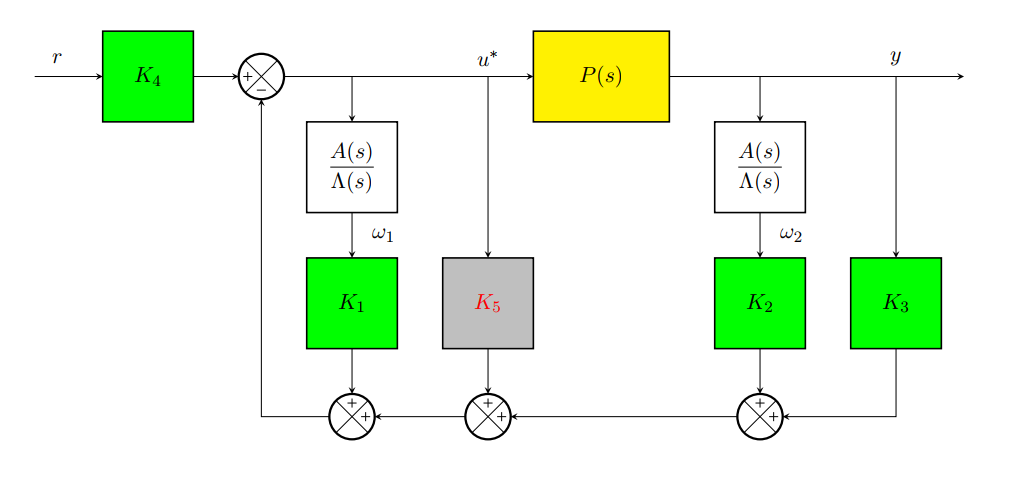
\includegraphics[width=15cm]{figs/mrac.png}
  \caption{Estrutura MIMO MRAC.}
  \label{mrac} 
\end{figure}

Comparando com o caso SISO, $\text{sign}(D)$ substitui $\text{sign}(K_p)$ e a
nova lei de controle � $u = \Omega^\intercal\Theta$. Por�m temos que garantir a
condi��o $M(s)S$ SPR. Temos que $M(s)S$ � SPR $\iff AP+PA=-2Q<0$ e $PS=I$,
onde $\{A,B,C\}$ � uma realiza��o de $M(s)S$. Para o caso $n^* = 1$, temos:

\begin{align}
M(s) &= \begin{bmatrix}
\frac{1}{s+a_1} & 0\\
0 & \frac{1}{s+a_2}
\end{bmatrix} \\
\nonumber A &= \begin{bmatrix}
-a_1 & 0\\
0 & -a_2
\end{bmatrix}
\end{align}

Se $a_1 = a_2 = a$, ent�o $M(s)S = \frac{1}{s+a}S$. 

\begin{align}
P = S^{-1} &= (L_pD_+L_p^\intercal)^{-1} = \begin{bmatrix}
d_1 & d_1l_1\\
d_1l_1 & d_2+d_1l_1^2
\end{bmatrix}^{-1} = \begin{bmatrix}
\frac{1}{d_1}+\frac{l_1^2}{d_2} & -\frac{l_1}{d_2} \\
-\frac{l_1}{d_2} & \frac{1}{d_2}
\end{bmatrix}
\end{align}

\begin{align}
Q &= - frac{PA+AP}{2} = \begin{bmatrix}
\frac{a}{d_1}+\frac{al_1^2}{d_2} & -\frac{l_1a}{d_2}\\
-\frac{l_1}{d_2} & \frac{a}{d_2}
\end{bmatrix}\\
\nonumber \text{det}(Q) &= -\frac{a^2}{d_1d_2}
\end{align}
%
Portanto, $Q<0$ para todo S. Igual ao caso SISO (notas de aula), por Lyapunov
podemos chegar na lei de adapta��o:

\begin{equation}
\dot{\Theta}(t) = -\textrm{sign}[D] \, \Gamma \, \Omega(t) \, e(t),
\end{equation}

onde  $D = \text{diag}\left\{ d_1I_1, d)2I_2, \ldots , d_mI_m\right\}$

o erro converge assintoticamente para zero, em que $\Gamma =
\Gamma^\intercal > 0$ � uma matriz de ganhos positiva definida.

Neste trabalho, ser�o consideradas plantas de primeira e segunda ordens com grau
relativo 1 ($n^*=1$). Iremos simular e discutir o comportamento do erro e das
sa�das para varia��es das condi��es iniciais dos par�metros estimados
($\theta(0)$) e da planta ($y(0)$), do ganho de adapta��o $\Gamma$ e para
diferentes par�metros da planta e modelo.

\section{Implementa��o}

Foram considerados dois casos: caso em que $K_p$ � desconehcido; e caso em que
todos os par�metros da planta s�o desconhecidos.

\subsection{Caso onde apenas $K_p$ � desconhecido}
\lstinputlisting[style=myMatlab]{../matlab/1/mrac.m} 

\subsection{Caso onde todos os par�metros s�o desconhecidos}
\lstinputlisting[style=myMatlab]{../matlab/2/mrac.m}
%---------------------------------------------------------------------
\section{Resultados das simula��es}

%Simula��o utilizando \HI{\texttt{Matlab/Simulink}}.

%\subsection{Gradiente Normalizado}

Nas simula��es, procuramos avaliar o comportamento do sistema para as seguintes condi��es:
%
\begin{enumerate*}[label=(\roman*)]
\item condi��es iniciais $\theta(0)$ e $y(0)$;
\item Par�metros da planta e do modelo;
\item ganho de adapta��o $\Gamma$.
\end{enumerate*}

Apresentaremos os resultados obtidos atrav�s de simula��es no ambiente \HI{\texttt{Matlab/Simulink}} e os discutiremos na pr�xima se��o.

\subsection{Simula��o \#1}

Inicialmente, verificamos o comportamento do sistema para varia��es no \textbf{par�metro de adapta��o} $\Gamma$.

\bigskip

\textbf{\underline{Simula��o 1.1}: sistema de 2$^\text{a}$ ordem}
%
\begin{align*}
  y &= \frac{s+1}{s^2+4s+4}u \,, &  y_m &=
  \frac{1}{s+1}r\,, & A_0 &= 1,\\ \theta(0) &= \mathbf{0} \,, & y(0) &= \textbf{0} \,, &
  \gamma &= \HI{20} \textbf{I}_4 \,, \, \textrm{e} \, \HI{1} \, \textbf{I}_4\,, \\ r &=
  10\textrm{sin}(0.635t) + 25\textrm{sin}(4.567t) \, .
\end{align*}

\begin{figure}[H]
  \centering
  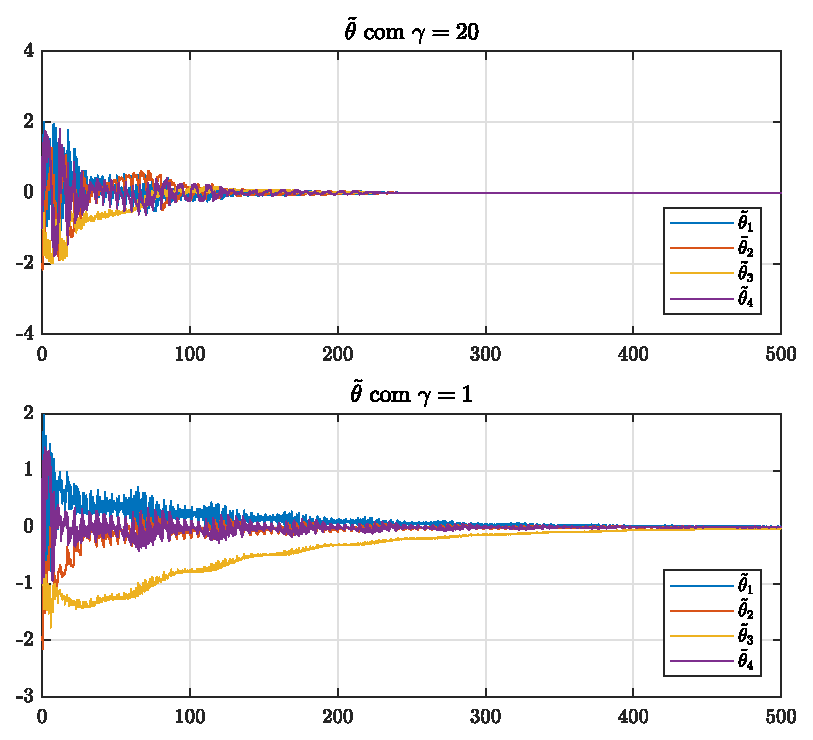
\includegraphics[width=12cm]{figs/tiltheta/sim02_gamma20gamma1.eps}
\end{figure}

\begin{figure}[H]
  \centering
  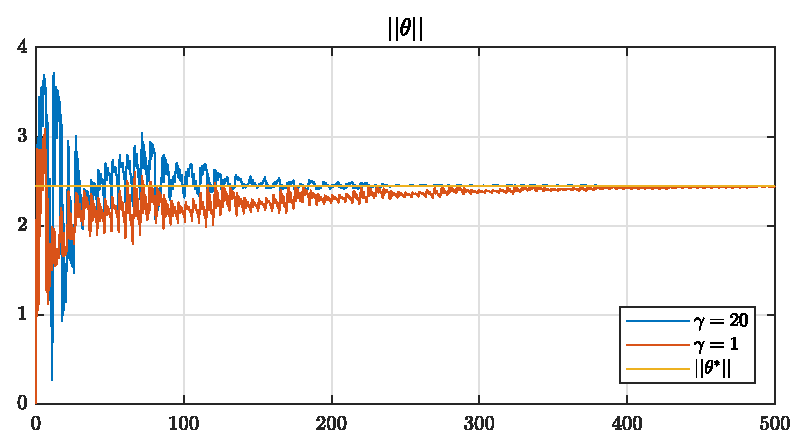
\includegraphics[width=12cm]{figs/modtheta/sim02_gamma20gamma1.eps}
\end{figure}

\begin{figure}[H]
  \centering
  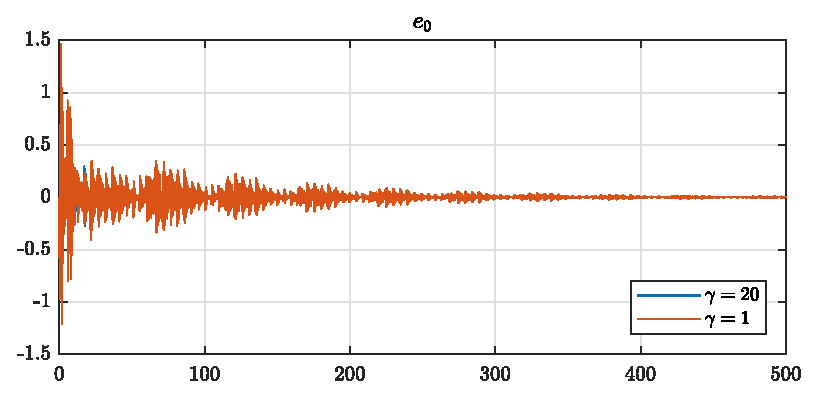
\includegraphics[width=12cm]{figs/e0/sim02_gamma20gamma1.eps}
\end{figure}

\bigskip

\textbf{\underline{Simula��o 1.2}: sistema de 3$^\text{a}$ ordem}
%
\begin{align*}
  y &= \frac{s^2+2s+1}{s^3+6s^2+12s+8}u \,, &  y_m &=
  \frac{1}{s+1}r\,, & A_0 &= 1,\\ \theta(0) &= \mathbf{0} \,, & y(0) &= \textbf{0} \,, &
  \gamma &= \HI{20} \textbf{I}_6 \,, \, \textrm{e} \, \HI{1} \, \textbf{I}_6\,, \\ r &= 10\textrm{sin}(t) + 25\textrm{sin}(2.1t) + 10\textrm{sin}(3.5t) \, .
\end{align*}

\begin{figure}[H]
  \centering
  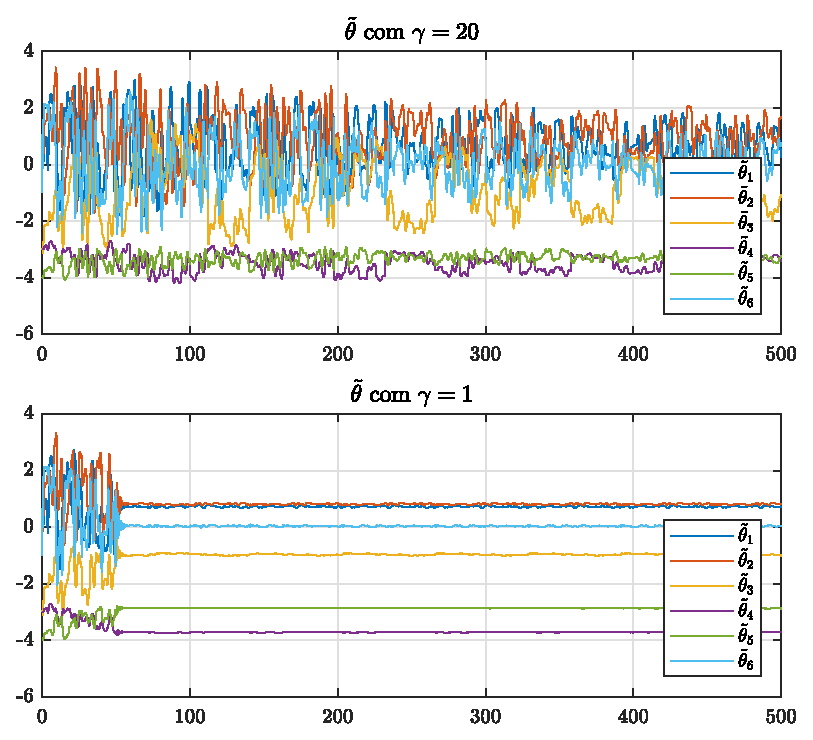
\includegraphics[width=12cm]{figs/tiltheta/sim03_gamma20gamma1.eps}
\end{figure}

\begin{figure}[H]
  \centering
  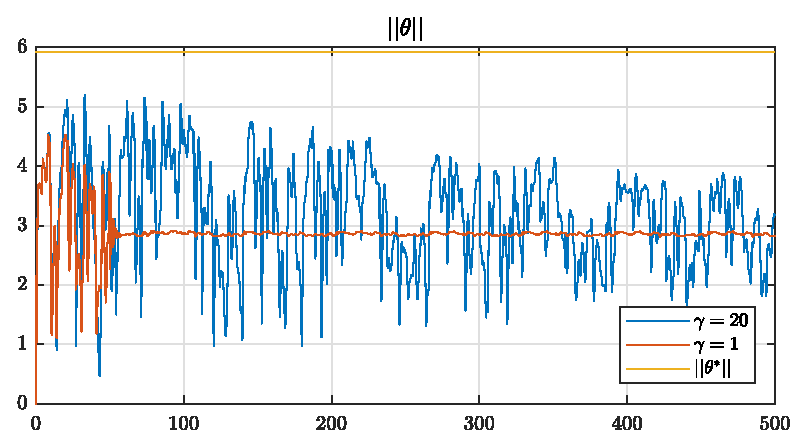
\includegraphics[width=12cm]{figs/modtheta/sim03_gamma20gamma1.eps}
\end{figure}

\begin{figure}[H]
  \centering
  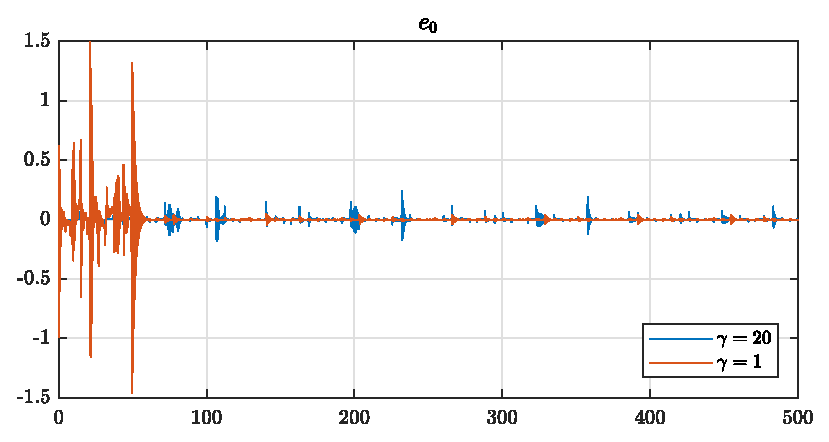
\includegraphics[width=12cm]{figs/e0/sim03_gamma20gamma1.eps}
\end{figure}

%---------------------------------------------------------------------

\subsection{Simula��o \#2}

Verificamos agora o comportamento do sistema para varia��es na \textbf{condi��o inicial} $y(0)$.

\bigskip

\textbf{\underline{Simula��o 2.1}: sistema de 2$^\text{a}$ ordem}
%
\begin{align*}
  y &= \frac{s+1}{s^2+4s+4}u\,,  &  y_m &= \frac{1}{s+1}r\,, & A_0 &= 1,\\ \theta(0) &= \mathbf{0} \,, & y(0) &= \HI{$\mathbf{0}$ \,, $\mathbf{10}$} \,, &
  \gamma &= 20 \, \textbf{I}_4\,, \\ r &= 10\textrm{sin}(0.635t) + 25\textrm{sin}(4.567t) \, .
\end{align*}

\begin{figure}[H]
  \centering
  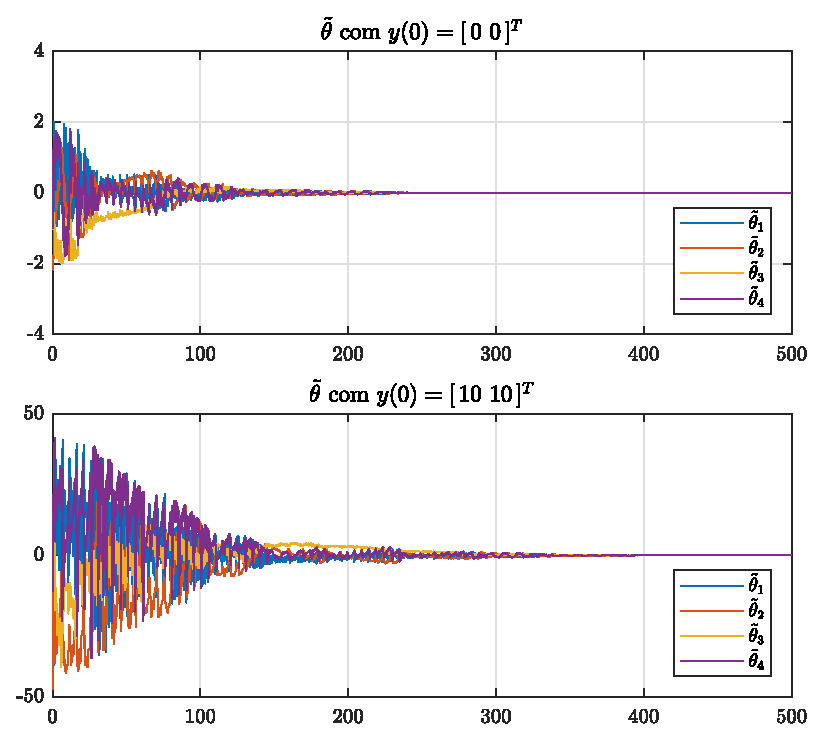
\includegraphics[width=12cm]{figs/tiltheta/sim02_y01y02.eps}
\end{figure}

\begin{figure}[H]
  \centering
  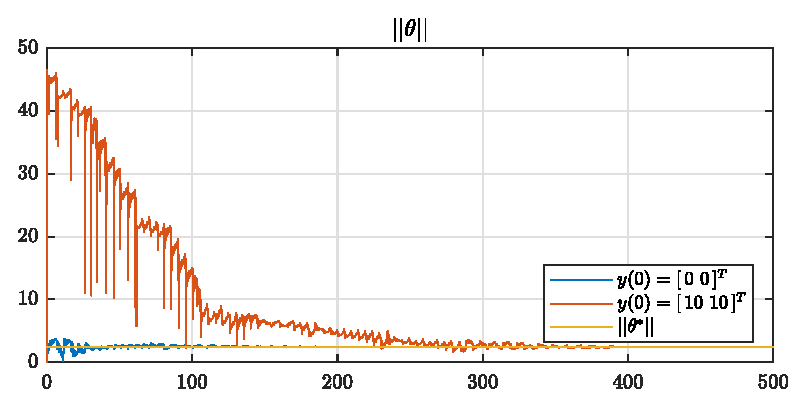
\includegraphics[width=12cm]{figs/modtheta/sim02_y01y02.eps}
\end{figure}

\begin{figure}[H]
  \centering
  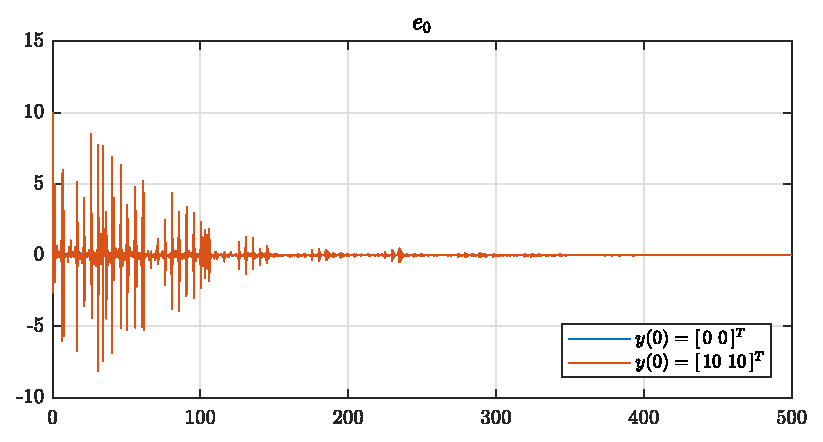
\includegraphics[width=12cm]{figs/e0/sim02_y01y02.eps}
\end{figure}

\bigskip

\textbf{\underline{Simula��o 2.2}: sistema de 3$^\text{a}$ ordem}
%
\begin{align*}
  y &= \frac{s^2+2s+1}{s^3+6s^2+12s+8}u \,, &  y_m &=
  \frac{1}{s+1}r\,, & A_0 &= 1,\\ \theta(0) &= \mathbf{0} \,, & y(0) &= \HI{$\mathbf{0}$ \,, $\mathbf{10}$} \,, &
  \gamma &= 20 \textbf{I}_6 \,, \\ r &= 10\textrm{sin}(t) + 25\textrm{sin}(2.1t) + 10\textrm{sin}(3.5t) \, .
\end{align*}

\begin{figure}[H]
  \centering
  \includegraphics[width=12cm]{figs/tiltheta/sim03_y01y02.eps}
\end{figure}

\begin{figure}[H]
  \centering
  \includegraphics[width=12cm]{figs/modtheta/sim03_y01y02.eps}
\end{figure}

\begin{figure}[H]
  \centering
  \includegraphics[width=12cm]{figs/e0/sim03_y01y02.eps}
\end{figure}

% -----------------------------------------------------------------------------

\subsection{Simula��o \#3}

Verificamos o comportamento do sistema para varia��es na \textbf{fun��o de transfer�ncia da planta} $P(s)$.

\bigskip

\textbf{\underline{Simula��o 3.1}: sistema de 2$^\text{a}$ ordem}
%
\begin{align*}
  y &= \HI{$\frac{s+1}{s^2+4s+4}u$}\,, \HI{$\frac{2s+4}{s^2+7s+12}u$}\,,  &  y_m &=
  \frac{1}{s+1}r\,, & A_0 &= 1,\\ \theta(0) &= \textbf{0} \,, & y(0) &= \textbf{0} \,, &
  \gamma &= 20 \, \textbf{I}_4\,, \\ r &= 10\textrm{sin}(0.635t) + 25\textrm{sin}(4.567t) \, .
\end{align*}

\begin{figure}[H]
  \centering
  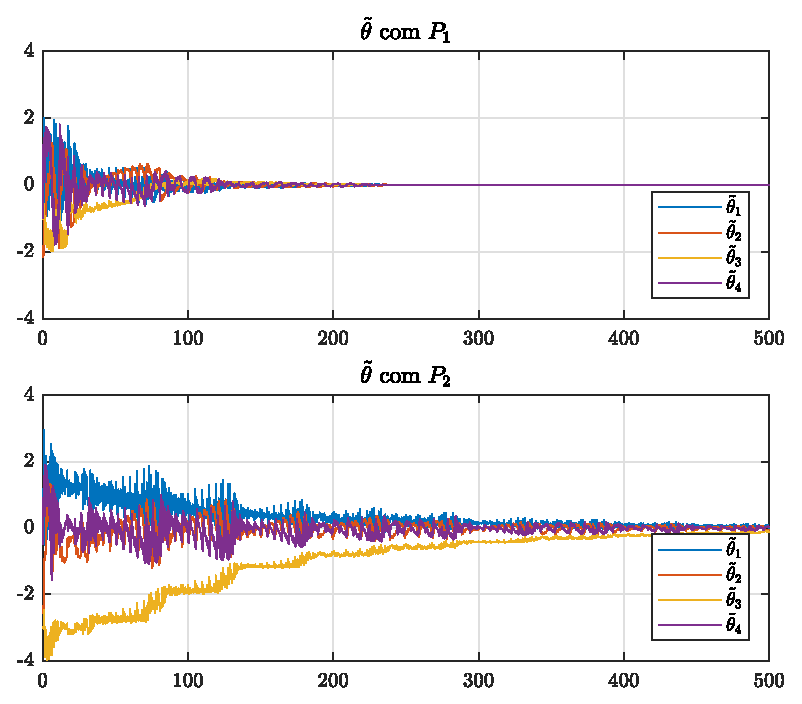
\includegraphics[width=12cm]{figs/tiltheta/sim02_P1P2.eps}
\end{figure}

\begin{figure}[H]
  \centering
  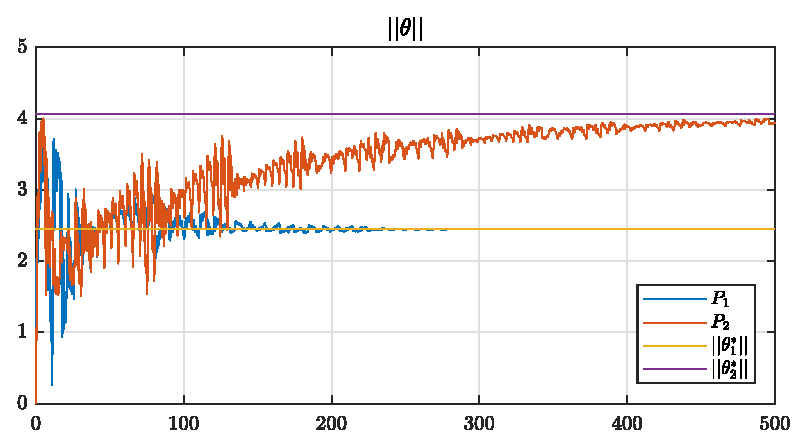
\includegraphics[width=12cm]{figs/modtheta/sim02_P1P2.eps}
\end{figure}

\begin{figure}[H]
  \centering
  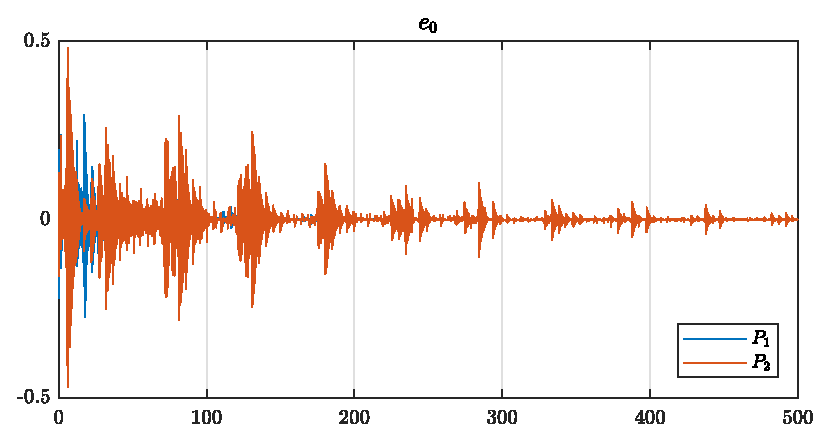
\includegraphics[width=12cm]{figs/e0/sim02_P1P2.eps}
\end{figure}

\textbf{\underline{Simula��o 3.2}: sistema de 3$^\text{a}$ ordem}
%
\begin{align*}
  y &= \HI{$\frac{s^2+2s+1}{s^3+6s^2+12s+8}u$}\,, \HI{$\frac{2s^2+16s+32}{s^3+6s^2+11s+6}u$}\,,  &  y_m &=
  \frac{1}{s+1}r\,, & A_0 &= 1,\\ \theta(0) &= \textbf{0} \,, & y(0) &= \textbf{0} \,, &
  \gamma &= 20 \, \textbf{I}_6\,, \\ r &= 10\textrm{sin}(t) + 25\textrm{sin}(2.1t) + 10\textrm{sin}(3.5t) \, .
\end{align*}

\begin{figure}[H]
  \centering
  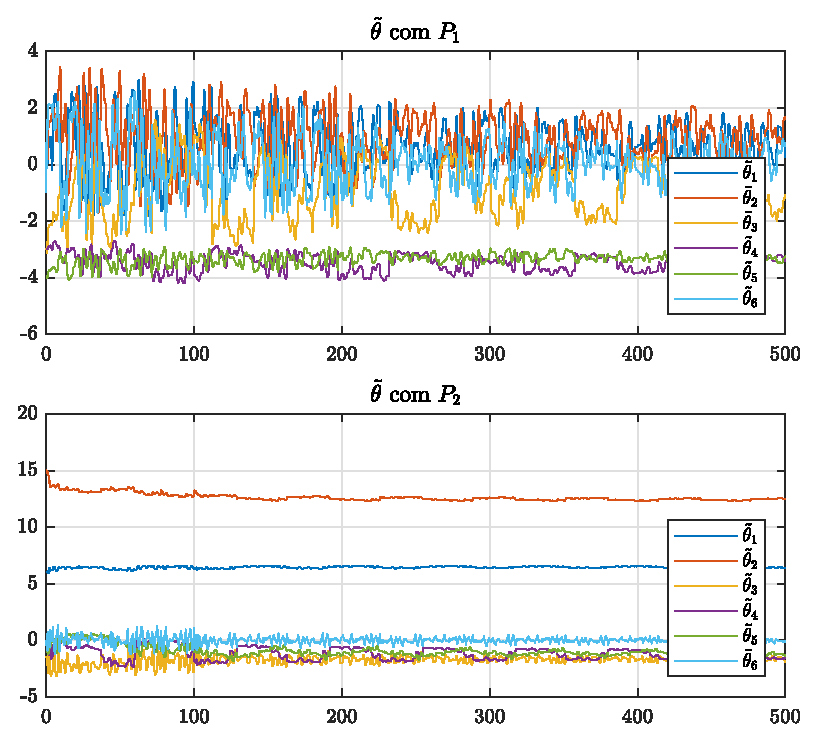
\includegraphics[width=12cm]{figs/tiltheta/sim03_P1P2.eps}
\end{figure}

\begin{figure}[H]
  \centering
  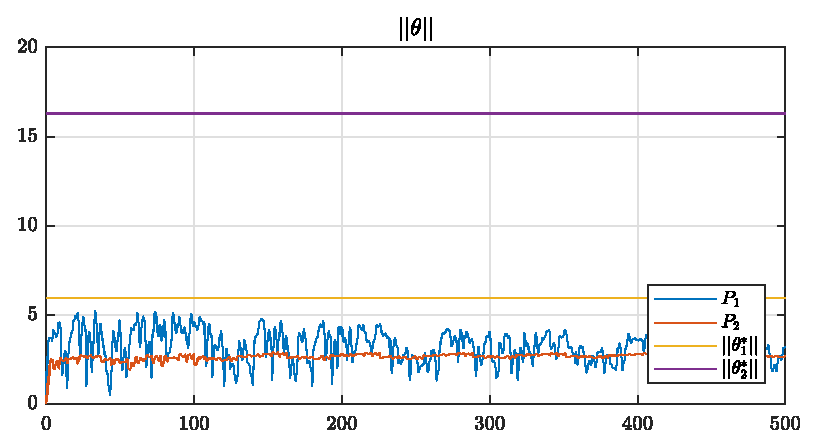
\includegraphics[width=12cm]{figs/modtheta/sim03_P1P2.eps}
\end{figure}

\begin{figure}[H]
  \centering
  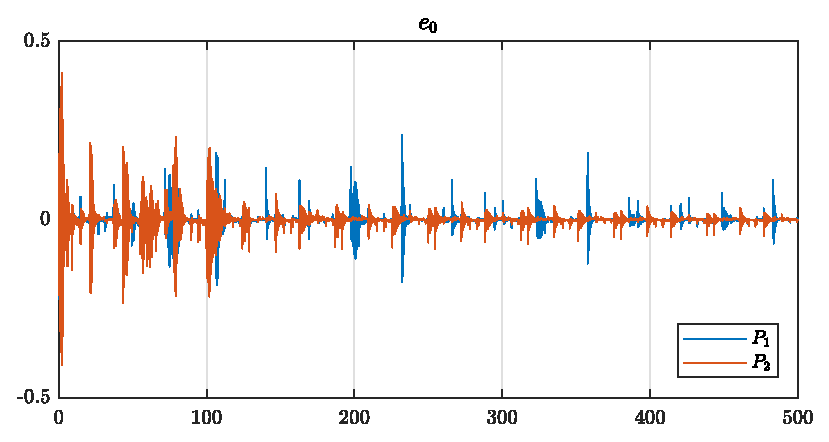
\includegraphics[width=12cm]{figs/e0/sim03_P1P2.eps}
\end{figure}

% -----------------------------------------------------------------------------

\subsection{Simula��o \#4}

Verificamos o comportamento do sistema para varia��es na \textbf{fun��o de transfer�ncia do modelo de refer�ncia} $P_m(s)$.

\bigskip

\textbf{\underline{Simula��o 4.1}: sistema de 2$^\text{a}$ ordem}
%
\begin{align*}
  y &= \frac{s+1}{s^2+4s+4}u \,,  &  y_m &= \HI{$\frac{1}{s+1}r$}\,, \HI{$\frac{s+1}{s^2+5s+6}r$ (n�o SPR)}\,, & A_0 &= 1,\\ \theta(0) &= \textbf{0} \,, & y(0) &= \textbf{0} \,, &
  \gamma &= 20 \, \textbf{I}_4\,, \\ r &= 10\textrm{sin}(0.635t) + 25\textrm{sin}(4.567t) \, .
\end{align*}

\begin{figure}[H]
  \centering
  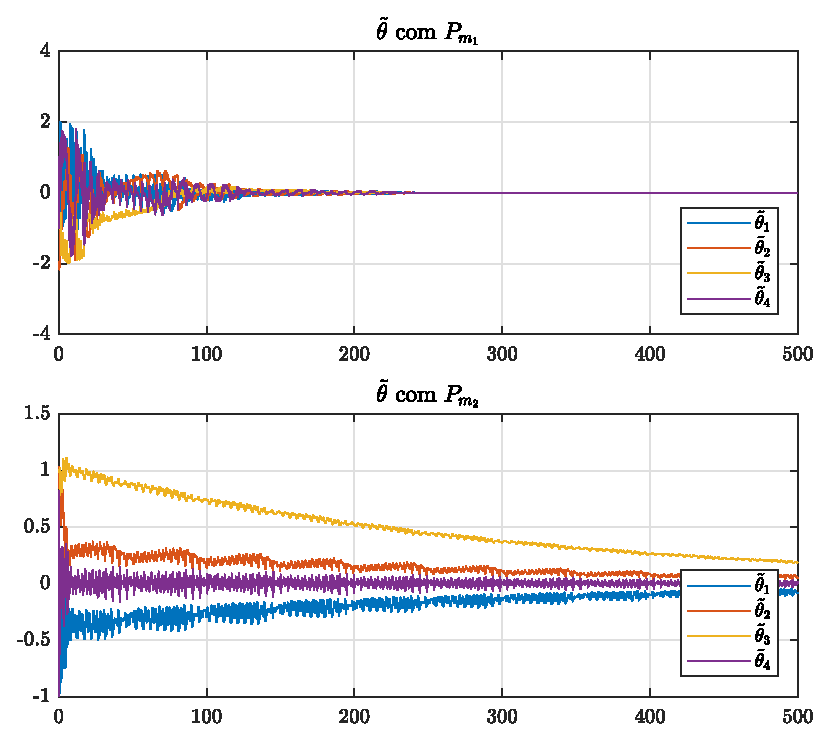
\includegraphics[width=12cm]{figs/tiltheta/sim02_Pm1Pm2.eps}
\end{figure}

\begin{figure}[H]
  \centering
  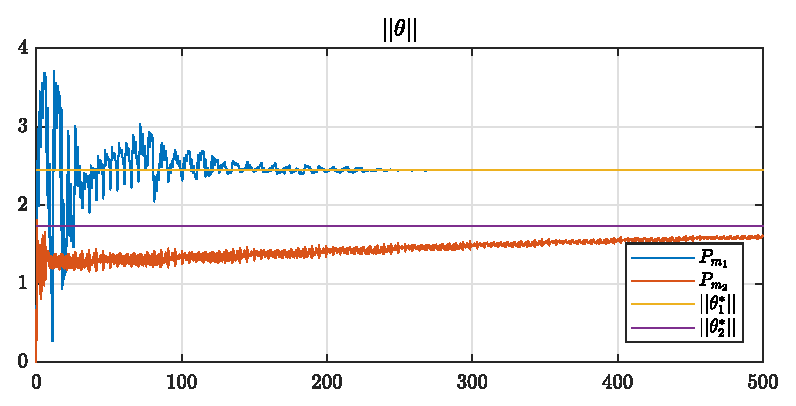
\includegraphics[width=12cm]{figs/modtheta/sim02_Pm1Pm2.eps}
\end{figure}

\begin{figure}[H]
  \centering
  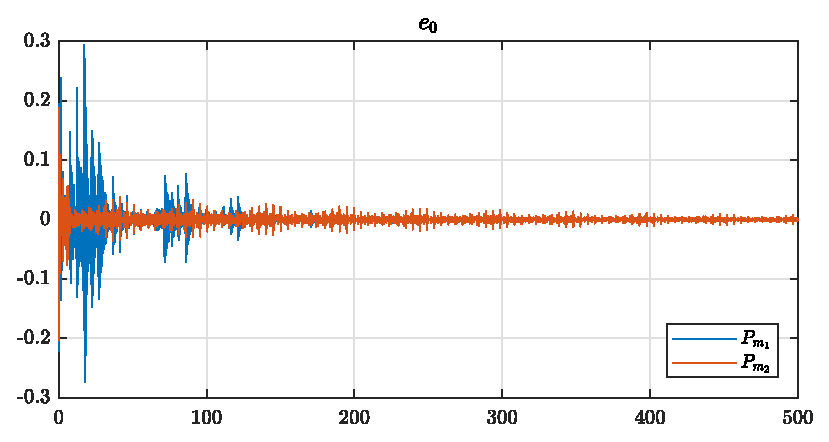
\includegraphics[width=12cm]{figs/e0/sim02_Pm1Pm2.eps}
\end{figure}

\textbf{\underline{Simula��o 4.2}: sistema de 3$^\text{a}$ ordem}
%
\begin{align*}
  y &= \frac{s^2+2s+1}{s^3+6s^2+12s+8}u \,,  &  y_m &= \HI{$\frac{1}{s+1}r$}\,, \HI{$\frac{s^2+2s+1}{s^3+5.5s^2+8.5s+3}r$ (n�o SPR)}\,, & A_0 &= 1,\\ \theta(0) &= \textbf{0} \,, & y(0) &= \textbf{0} \,, &
  \gamma &= 20 \, \textbf{I}_6\,, \\ & & r &= 10\textrm{sin}(t) + 25\textrm{sin}(2.1t) + 10\textrm{sin}(3.5t) \, .
\end{align*}

\begin{figure}[H]
  \centering
  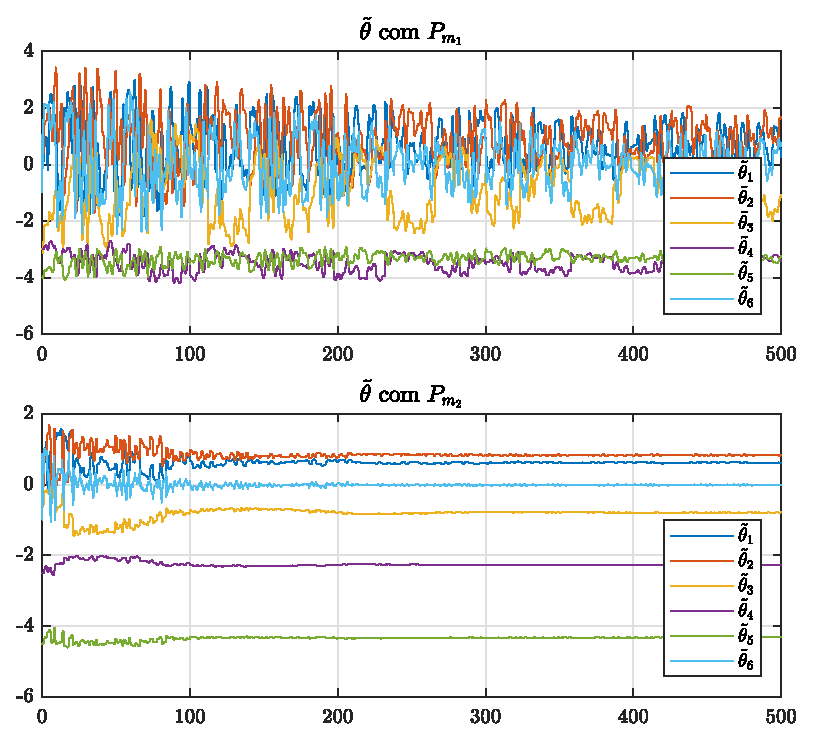
\includegraphics[width=12cm]{figs/tiltheta/sim03_Pm1Pm2.eps}
\end{figure}

\begin{figure}[H]
  \centering
  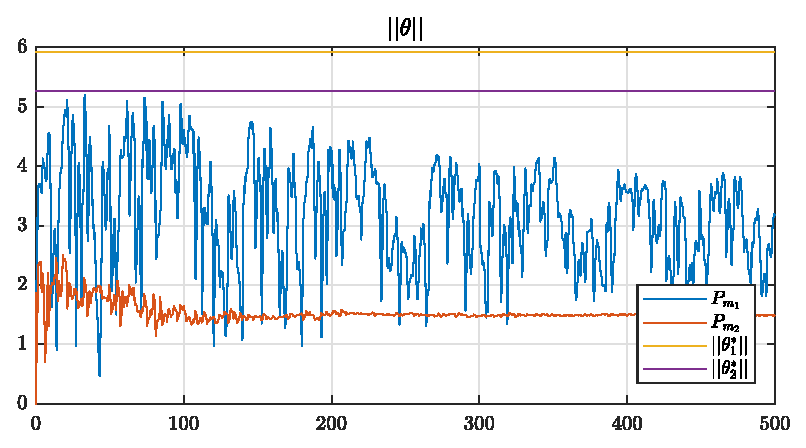
\includegraphics[width=12cm]{figs/modtheta/sim03_Pm1Pm2.eps}
\end{figure}

\begin{figure}[H]
  \centering
  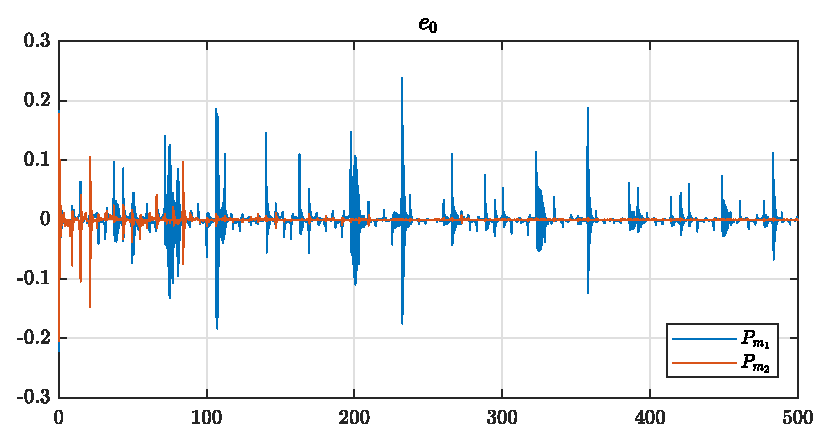
\includegraphics[width=12cm]{figs/e0/sim03_Pm1Pm2.eps}
\end{figure}
 \newpage
%---------------------------------------------------------------------
\section{Discuss�o}

Neste trabalho, s�o abordados sistemas com duas entradas e duas sa�das (MIMO) e
plantas de primeira e segunda ordem com grau relativo 1. O filtro foi definido como mais
simples poss�vel.

Comparativamente, quando apenas $K_p$ � desconhecido (5 par�metros), o erro
converge rapidamente para zero, aproximadamente 15 segundos, usando ganhos de adapta��o
$\Gamma$ entre 1 e 10. O erro leva mais tempo para convergir para zero quando
todos os par�metros s�o desconhecidos (17 par�metros), aproximadamnte 60
segundos, com ganho de adapta��o 20, e o tempo de
simula��o tamb�m � bem mais elevado, pois a \textit{ode} calcula a derivada de
17 par�metros.

A \textbf{simula��o \#1} mostra o comportamento do sistema para varia��es no
ganho de adapta��o $\Gamma$. Aumentar o ganho de
adapta��o garante converg�ncia mais r�pida, por�m mais oscila��es.

A \textbf{simula��o \#2} mostra o comportamento do sistema para varia��es nas
condi��es iniciais da planta $y(0)$. O sistema oscila mais para condi��es
iniciais da planta longe de zero. O transit�rio, por�m, foi menor para os
sistemas com condi��o inicial diferente de zero. Isso ocorre, pois os par�metros
entraram rapidamente em quadratura com o vetor de regressor.

A \textbf{simula��o \#3} mostra o comportamento do sistema para varia��es no
ganho de adapta��o na planta. O deslocamento ($\phi$) n�o alterou muito o
ressultado. Vale observar o problema quando $\phi  > \frac{\pi}{2}$ (simula��o
3.1 quando apenas $K_p$ �  dessconhecido), pois o sistema apresenta
comportamento inst�vel j� que os sinais de $D$ s�o opostos. Para o caso em que
todos os  par�metros s�o  desconehcidos, foi escolhida uma planta mais r�pida e
dif�cil de ser controlada, e o controlador foi capaz de estabilizar. 

A \textbf{simula��o \#4} mostra o comportamento do sistema para varia��es no
modelo. Modelos mais r�pidos apresentaram maiores oscila��es e exigiram mais
tempo para convergir.
 
%---------------------------------------------------------------------
%\bibliographystyle{agsm}
%\bibliography{bib,coe736}

%---------------------------------------------------------------------
\end{document}
